\chapter{Pytropos (Analysis Implementation)}%
\label{pytropos-analysis-implementation}

Pytropos\footnote{There is an old trend where programs, companies and
  anything that could be named was named after some mythological
  creature from an ancient civilization. Thus, why could not this work
  also have a proper ancient-based name. Pytropos comes from the merge
  of Python and Atropos. In the Greek mythology, Atropos was one of the
  three goddesses of fate who decided on the lifes of humans, she was
  the goddess of death and the one who cut the thread of life.} is the
Abstract Interpreter implemented in this work. The interpreter follows
the rules exposed in the previous chapter.

This chapter is divided into two parts. In the first part, we explore
how is Pytropos built, a brief history and some internal details. The
second part is a small guide on how to interpret Pytropos output over a
couple of different examples.

\section{The big picture}\label{the-big-picture}

{\missingfigure{How the system works in an image}}

Pytropos works in a similar way as any other Python interpreter does. It
reads code and executes it expression by expression. Its main difference
to CPython is that it does not transform code into bytecode to execute
but it wraps code before it is transformed into CPython bytecode. The
code is wrapped to use a library that implements the semantics of the
Abstract Interpreter.

Similar to how Python works, Pytropos can not only \enquote{run}
individual files, but also offers a REPL (Read-eval-print loop) to check
small portions of code.

\section{Wrapped code + libs + interpreter vs.~from scratch interpreter}%
\label{wrapped-code-libs-interpreter-vs.from-scratch-interpreter}

{\inlinetodo{add little note on what means to write an interpreter from
scratch}}

\textcite{ortin_towards_2015} show how to build a Static Type Analysis
by rewriting code to operate with the types of values rather than with
the values, i.e.~the result of executing the code is not some values but
some types. For example, consider the following small piece of code:

\begin{pythoncode}
a = 2 + 4
b = a + "yep"  # this will fail
c = a / 2
\end{pythoncode}

Notice that how even though the piece of code fails to run successfully,
we can determine the types of all variables. \pycode|a| has type
\pycode|int|, \pycode|b| has no type as it cannot be
computed, and \pycode|c| has type \pycode|float| because the
division of \pycode|int|s in Python 3 gives us back a \pycode|float|.

We can build a library that operates on types (rather than values) and
then we can rewrite the piece of code above into:

\begin{pythoncode}
import typeops as to
a = to.add(int, int)
b = to.add(a, str)
c = to.div(a, int)
\end{pythoncode}

If the library has properly defined the methods \pycode|add| and
\pycode|div|, we can be sure that the code will run without any error.
Notice that the library is able to find type mismatches by embedding
checks in the functions \pycode|add| and \pycode|div|. The library can,
effectively, perform Static Analysis on a piece of code.

Pytropos is implemented following the same strategy: a library that
operates over abstract values, and a transformation procedure that takes
the code and wraps it to use the library. The final step is to run the
wrapped code and collect the generated errors\footnote{This strategy has
  been applied on the past for similar purposes, reuse of
  infrastructure. It was used by \textcite{lauko_symbolic_2018} for
  symbolic computation of LLVM bytecode.
  %\inlinetodo{actually I'm not aware of any other example where this has been done :S}
  }.

The main advantage of translating code into wrapped code is the reuse of
infraestructure. One does not need to write all the infraestructure that
an interpreter needs. Pytropos does not implement its own call system,
heap management or garbage collection. All of it is managed by the
underlying Python implementation where the code is executed.

Nevertheless, this approach has three main disadvantages. First, all
operations, function calls, attribute access, subscript access and the
whole Python semantics, must be coded into the library and in the
transformation function. Second, the place where any operation has
occurred must be preserved too, otherwise it is impossible to find where
an error has occurred. Finally, all variable access must be wrapped too,
because accessing to an undefined variable must stop execution.
Consequently, the transformation does not produce a simple,
human-readable output. We can run Pytropos with the small code above as
input and will get:

\begin{pythoncode}
import pytropos.internals as pt
st = pt.Store()
pt.loadBuiltinFuncs(st)
fn = 'test.py'
st[('a', ((1, 0), fn))] = pt.int(2).add(pt.int(4), pos=((1, 4), fn))
st[('b', ((2, 0), fn))] = st[('a', ((2, 4), fn))].add(pt.str('yep'), pos=((2, 4), fn))
st[('c', ((3, 0), fn))] = st[('a', ((3, 4), fn))].truediv(pt.int(2), pos=((3, 4), fn))
\end{pythoncode}

Not as nice as the first example.

Pytropos started out from the same idea as \textcite{ortin_towards_2015}
but it differs on its principal goal. Pytropos goal was not to perform
Static Type Analysis but Static Value Analysis. After working for three
months on a prototype, it became blatantly clear that trying to wrap the
code naïvely did not work very well, i.e.~the code was a hacky and not
very resilient. The library and transformation needed to be based on a
solid theoretical framework.

Enter Abstract Interpretation. Abstract Interpretation offers the ideal
framework for Static Value Analysis, it is well understood, with solid
theory and extensive work on it has been done for the last four decades.

\textcite{ortin_towards_2015} strategy alone may still be a good idea
for Static Type Analysis, but it may not work without a framework to
glue together the semantics of the languages with those of the analysis.
Their legacy to Pytropos is the reuse of Python infrastructure by
wrapping the code and not building an interpreter from scratch.

\section{Assumptions}\label{assumptions}

Pytropos is limited to work only with Python 3.6 or higher. Pytropos
uses variable annotations to allow the user to specify the shape of
NumPy arrays when Pytropos is not able to \enquote{infer} their value.
Variable annotations were introduced on Python 3.6 \autocite{pep526}.

The goal of Pytropos is to warn the user when an operation will fail at
runtime. It is not a goal for Pytropos to verify the code and prove its
correctness (Pytropos is not a tool for verification).

Pytropos goal is not to replace MyPy, flake8, or any other static
analysis python tool\footnote{I use MyPy and flake8 in every project and
  I am thankful to the years of effort put into these amazing tools.
  Thank you guys!}. Pytropos is meant to be an aid for developers when
working with tensors.

Based on that, I present the main assumptions taken into account in the
implementation of Pytropos:

\begin{itemize}
\tightlist
\item
  The user wants as little warnings on the code as possible. Pytropos
  should warn the user for errors it is sure will occur at runtime.
\item
  The user cares only about the shape of tensors and not about the
  actual values a tensor holds.
\item
  If Pytropos is not able to infer the value of a variable, the user can
  (optionally) annotate the type/value of the variable. If the
  annotation is not preciser than the value that Pytropos has already
  inferred the inferred value will not change.
\end{itemize}

\section{Details on the guts}\label{details-on-the-guts}

To start with, I do not follow the structure defined in the previous
chapter for how elements are saved in memory. I did not explicitly
defined a Heap but make use of Python's heap. The main reason to not
define a custom Heap is the cost associated to it, especially the
definition of a Garbage Collector. The classes \texttt{AbstractMutVal}
and \texttt{Store}, the implementations of \texttt{Object\#} and
\texttt{G\#}, respectively, do not point to \texttt{Addr\#}s but they
point to \texttt{PythonValue}s directly (the implementations of
\texttt{Val\#}). The global scope, \texttt{Store}, is an object that
takes a \texttt{str} and returns a \texttt{PythonValue}. An
\texttt{Object\#}, \texttt{AbstractMutVal}, is an object that has an
associated type, operations and can point to any \texttt{PythonValue}.
In this way, the Pytropos resembles more the graph representation than
the classical Heap representation\footnote{Both representations are
  explained in detail in the previous chapter}.

The class \texttt{PythonValue} implements \texttt{Val\#} Abstract
Domain. A \texttt{PythonValue} is a wrapper around either a
\texttt{AbstractValue} or a \texttt{AbstractMutVal} (the implementations
of \texttt{PrimVal\#} and \texttt{Object\#}). Note that
\texttt{AbstractMutVal} subclasses \texttt{AbstractValue}, as well as do
\texttt{Int}, \texttt{Float}, \texttt{NoneType} and \texttt{Bool} which
implement \texttt{Int\#}, \texttt{Float\#}, \texttt{None\#} and
\texttt{Bool\#}, respectively, and also subclass from
\texttt{AbstractValue}.

\texttt{AbstractValue} is an abstract class that defines all the
operations supported (\pycode|+|, \pycode|*|, \ldots{}) by Pytropos, and
what it is required for a function call, subscript access and attribute
access. \texttt{AbstractValue}, in its turn, subclasses
\texttt{AbstractDomain} a abstract class that defines the methods every
Abstract Domain should have, namely \pycode|is_top()|, \pycode|join()|,
\pycode|top()| and \pycode|widen_op()|. \pycode|PythonValue| and
\texttt{Store}, unsurprisingly, also subclass \texttt{AbstractDomain}.

The figure below presents a class diagram showing the relationships
between the different components in Pytropos.

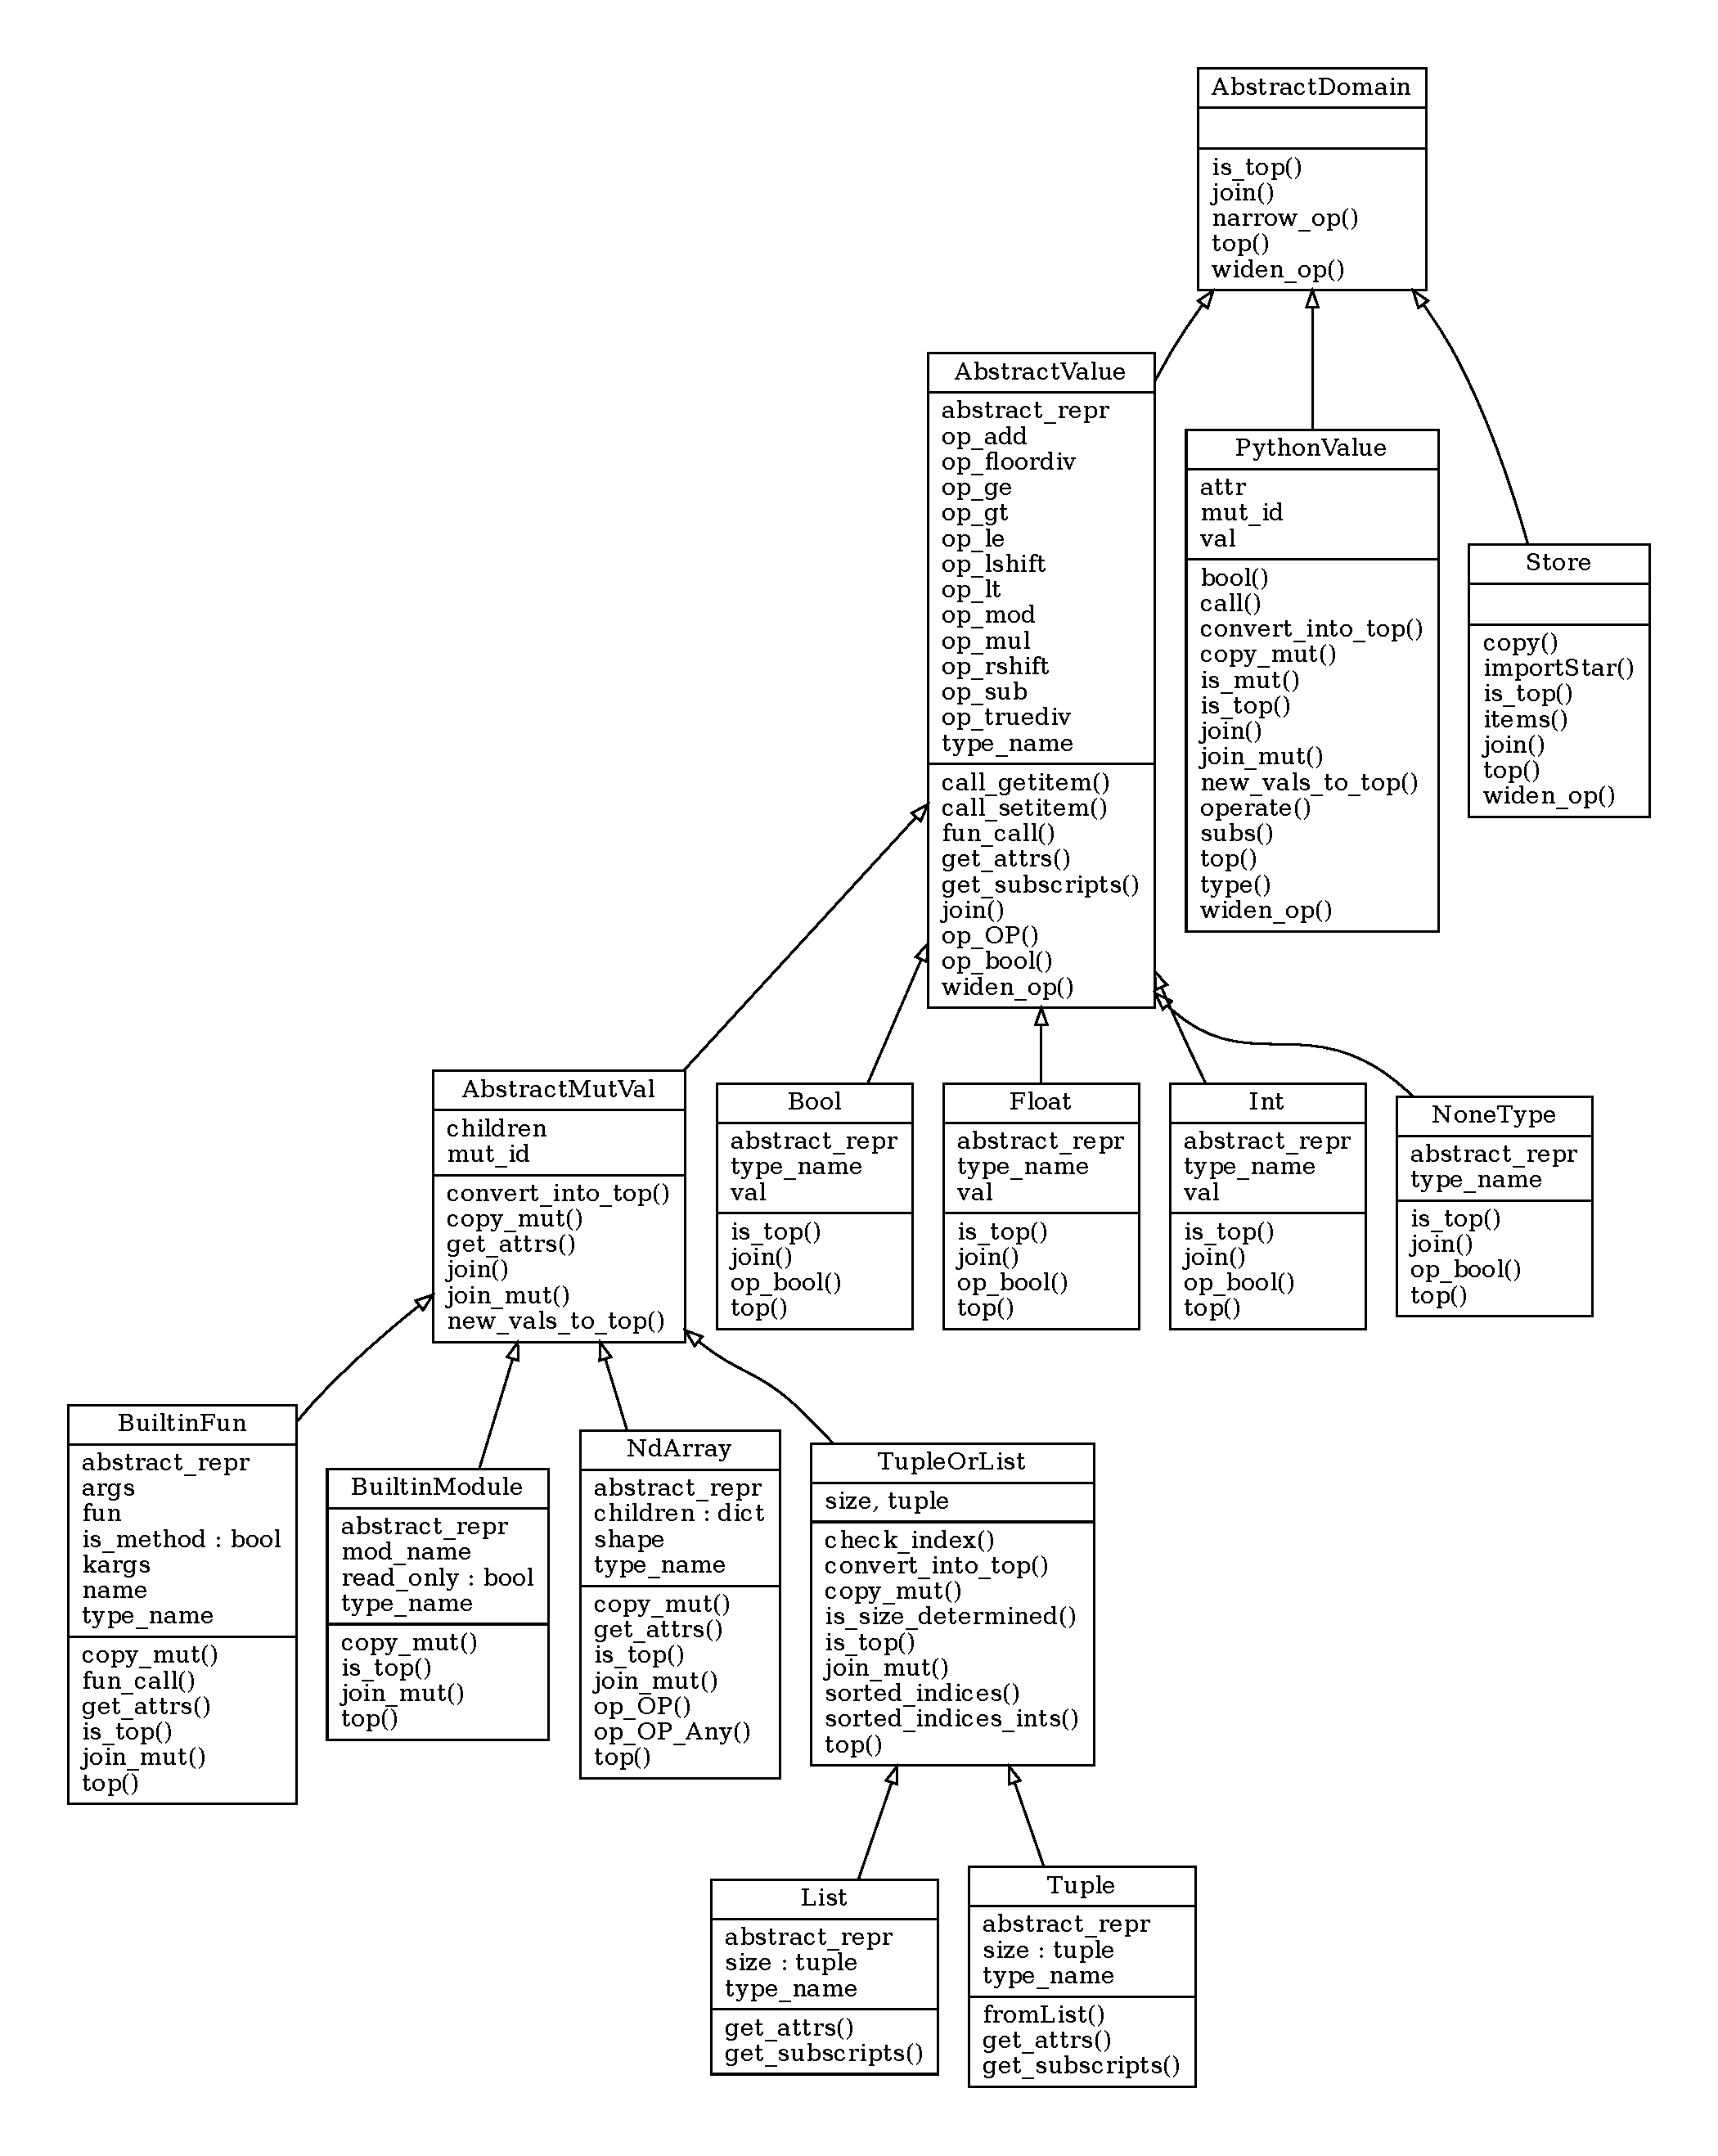
\includegraphics[width=0.8\textwidth]{figures/classes_Pytropos-small.pdf}
{\todo{add types to each attribute, and add hidden attributes like
\pycode+__getitem__+}}

\verb+<prim-callable>+ and all other
\texttt{Objects\#} are implemented by a subclass of
\pycode|AbstractMutVal|: \verb+<prim-callable>+
by \pycode|BuiltinFun|, \texttt{Module} objects by
\pycode|BuiltinModule|, \pycode|list|s by \texttt{List}, and
\pycode|tuple| by \texttt{Tuple}.

The implementation of the Abstract Interpreter also includes a class log that stores all
warnings generated in the abstract interpretation of the code.

{\inlinetodo{mention that \texttt{children} is the function
\texttt{Key\ -\textgreater{}\ Addr\ +\ Undefined}}} {\inlinetodo{mention
that \texttt{joinVal} is defined as \texttt{join\_mut} in
\texttt{PythonValue}, and \texttt{joinObject} is defined as
\texttt{join\_mut} in \texttt{AbstractMutVal}}}
